\chapter{背景}
\label{ch:background}
\section{検出対象の定義}
%第\ref{ch:introduction}章の通り,フェイクニュースの国際的にコンセンサスの取れた定義はない.
偽情報に類似した単語として、フェイクニュースがある。
フェイクニュースの国際的にコンセンサスの取れた定義はないものの、
英英辞典によっては定義を説明しようという取り組みもあり,コリンズ英英辞典では以下のように定義している\cite{collins_fake}.
\begin{quote}
    false, often sensational, information disseminated under the guise of news reporting
\end{quote}
ここでは,ニュース報道を模したセンセーショナルな虚偽の情報と定義している.
またコリンズ英英辞典は2017年を代表する単語として``Fake news''をWord of the Yearに選定している\cite{collins_word}.
一方,同じ出版会社から出されているコウビルド英英辞典では,次のように定義している\cite{collins_fake}.
\begin{quote}
    If you describe information as fake news, you mean that it is false even though it is being reported as news, for example by the media.
\end{quote}
この定義はある記事をフェイクニュースと指摘した場合,例えマスメディアが発信したニュースであろうと虚偽の情報が含まれることを意味するとしている.
コリンズ英英辞典と定義が異なるのは,虚偽の情報が含まれていると指摘したい時に使う状況を想定しているためとみられる.
このように、Fake newsという単語は同じ出版会社の英英辞典でも定義にゆらぎがみられる。

%misinformation, disinformation
フェイクニュース(Fake news)と近い意味を持つ言葉としてMis-informationとDis-information, そしてMal-informationがある.
これらの違いに関しては欧州評議会が出版したWardleとDerakhshanによる文書により、以下の\cref{fig:info}の通り真偽性と有害性によって分類されている\cite{wardle2017information}.

\begin{itemize}
    \item \textbf{Dis-information}: 虚偽の情報であり,個人や集団に対して有害な情報.
    \item \textbf{Mis-information}: 虚偽の情報である一方,悪意はなく有害性はない情報.%日本語における「誤報」や「誤情報」の定義に近い.
    \item \textbf{Mal-information}: 事実に基づいた情報であり,個人や集団に有害性を持たせるために用いられる情報.リークやヘイトスピーチなどが含まれる.
\end{itemize}

このうちDis-informationは欧州委員会の報告書でもdisinformationとして以下の通りに定義されている \cite{doi/10.2759/739290}。
初期の定義付けされた場合の単語に対して表記揺れが起きているが、ハイフン無しの表現が一般的となっている。

\begin{quote}
    all forms of false, inaccurate, or misleading information designed, presented and promoted to intentionally cause public harm or for profit
\end{quote}

日本語では、総務省で開催された研究会で disinformation への対訳として「偽情報」と表現している \cite{soumuDisinfo}。
また、2024年現在では政府広報より日本語の偽情報と誤情報の違いとして以下の定義付けがなされている \cite{gov2024}。

\begin{itemize}
    \item 偽情報とは?:
    人を混乱させ惑わすために意図的・意識的に作られたウソ、虚偽の情報
    \item 誤情報とは?:
    勘違いや誤解により拡散された間違った情報
\end{itemize}

本研究では,第\ref{ch:introduction}章の通り検出対象の定義をdisinformation・偽情報に該当するものとする.
また、偽情報の定義としては情報の内容に焦点を当てている点に留意する必要がある。
%また、本研究が検出対象とする情報の範囲から鑑みて、便宜上本論文では検出対象をdisinformation及び偽情報として表記する。

\begin{figure}[p]
    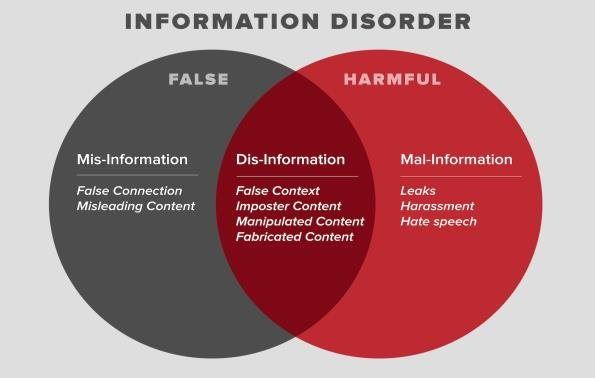
\includegraphics[width=\linewidth]{figures/fig_disorder.jpg}
    \caption{真実性・有害性による情報の分類と概要例\cite{wardle2017information}.}
    \label{fig:info}
\end{figure}

% \section{偽情報の詳細な分類}
% 一口に悪意によって意図的に作られた事実に反する情報と呼んでも,情報作成者の意図に悪意がどれだけ入ってくるかによって危険性は変わる.
% 偽情報が含まれるMis-informationとDis-informationは読者を欺こうとする悪意の度合いによって7種類に分けられるとしている\cite{wardle_2017}.
% 図\ref{fig:types}は左から右の順に以下を説明している.

% \begin{itemize}
%     \item \textbf{Satire or parody}: 皮肉あるいはパロディ.危害を加える意図はないが,読者を騙す可能性をもつ.最も悪意が少ない.
%     \item \textbf{False connection}: 見出しやキャプションが内容と乖離している.
%     \item \textbf{Misleading content}: ミスリード.情報を誤解を招く方向に利用している.
%     \item \textbf{False context}: 本当の内容が虚偽の文脈情報で共有されている.
%     \item \textbf{Imposter content}: 情報源として虚偽のものを使っている.
%     \item \textbf{Manipulated content}: 本当の情報や画像を操作して騙そうとしている.
%     \item \textbf{Fabricated content}: 新しい内容が完全に虚偽であり,騙して実害を与えようとしている.最も悪意が多い.
% \end{itemize}

% \begin{figure}[p]
%     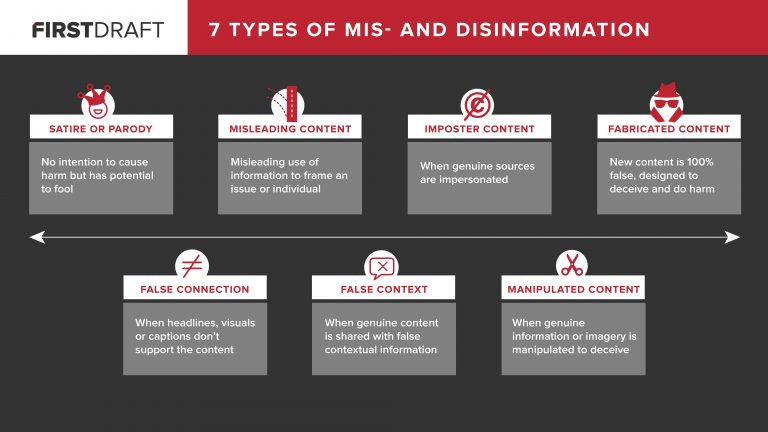
\includegraphics[width=\linewidth]{figures/fig_types.jpg}
%     \caption{誤情報(Mis-information, Dis-information)を作者の悪意の程度によって7種類に分類した図\cite{wardle_2017}.}
%     \label{fig:types}
% \end{figure}


\section{偽情報がもつ危険性}
近年でも、\cref{ch:introduction}で示した2022年のロシアによるウクライナ侵攻に関連した偽情報 \cite{evon_2022}に限らず、
2023年のパレスチナとイスラエルの戦争、そして2024年の能登半島地震といった社会情勢の変化に便乗した偽情報が投稿されている \cite{Press_2023,noto}。
これらの偽情報が拡散されることで発生する問題点は多岐にわたる。

\subsection{世論の操作}
偽情報の影響により世論が誘導された可能性がいくつか指摘されている.

例えば英インデペンデント紙は英国のEU離脱国民投票において,
図\ref{fig:leave}のように
「EUを離脱して毎週の拠出金3.5億ポンドをNHS(国民保険サービス)に供給しよう」といった主張\cite{merrick_2018}をはじめとする偽情報が選挙期間中に流布された結果,
離脱派の勝利に繋がった可能性が指摘されている\cite{grice_2017}.

また米ニューズウィーク誌によると2016年大統領選挙では,SNSプラットフォームで偽情報を含む情報によるターゲット広告を閉鎖的なコミュニティの中で発信することで,
有権者の支持を得ることに成功したと指摘している\cite{burleigh_2017}.

\begin{figure}[p]
    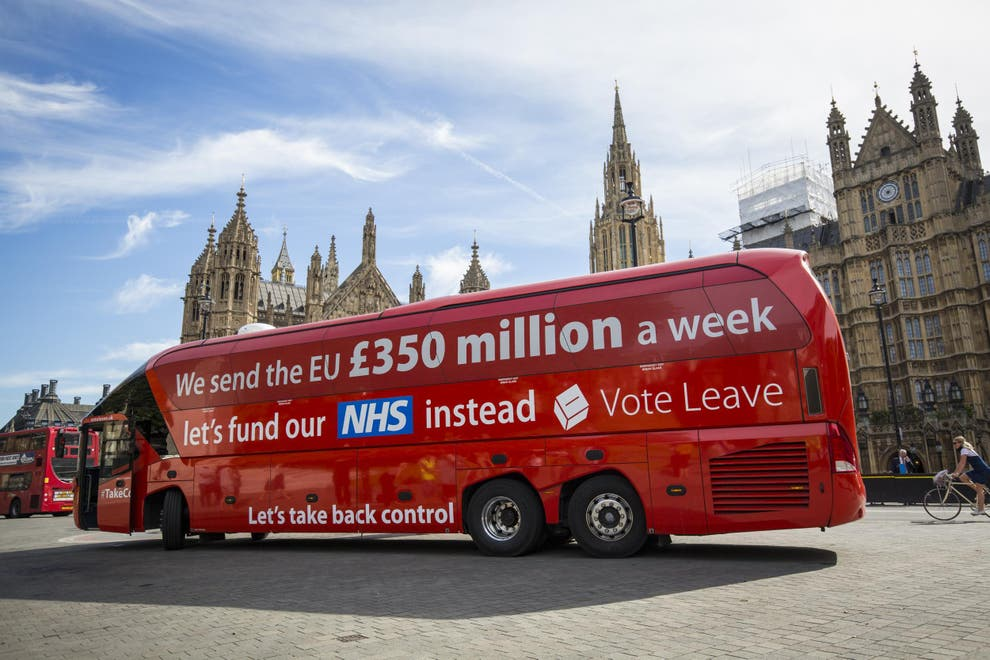
\includegraphics[width=\linewidth]{figures/fig_leave.jpg}
    \caption{英国でEU離脱の是非を問う国民投票の事前運動で出された広告.「EUを離脱すれば毎週払っている3.5億ポンドの拠出金をNHS(国民保険サービス)に供給できる」としているが,後にこれが誤りだった可能性を認めている\cite{merrick_2018}.}
    \label{fig:leave}
\end{figure}

このように、偽情報によって国民が正しい情報にアクセスできない場合、世論が操作され選挙結果にも影響を与えうる。
これを象徴するように、2024年の世界経済フォーラム年次総会(通称、ダボス会議)に先立って公開されたグローバルリスク報告書2024年版にて、今後2年間において最も重要・深刻なグローバルリスクとして「誤報と偽情報」(``Misinformation and disinformation'')を挙げたうえ、
今後10年間における重要さでも誤報と偽情報は全体の5位であるほか、学術領域から最も多く挙げられたグローバルリスクも誤報と偽情報と報告されている \cite{wef2024,wef2024_j}。
主な理由として、今後数年間に米国やインドといった超大国で選挙が予定されている点が挙げられている。

\subsection{事件への影響}
また実際に発生した事件に偽情報が影響を及ぼした事例も数多く報告されている.

例えば2016年米国大統領選挙期間中に「ワシントンDCの民主党支持者が経営するピザ屋は小児性愛者と児童売春の拠点となっており,ヒラリー・クリントン候補(当時)が関与している」という
偽情報が流布された結果,それを信じた者により銃撃事件に発展した \cite{agencies_2016}.
同じように偽情報が陰謀論の信奉者を増やした例としてQアノンが挙げられる.
これは「政財界とマスコミにエリートとして巣食う悪魔崇拝の小児性加害者たちに対して、トランプ前大統領は秘密の戦争を繰り広げている」という旨の内容である \cite{wendling_2021}が,
2021年1月に発生した米国議会襲撃事件にて,多くの信奉者が逮捕された \cite{hymes_mcdonald_watson_2021}.
このような陰謀論を人々に信じ込ませる手段として偽情報がSNSの発信を介して利用されている状況について,
WWW(ワールド・ワイド・ウェブ)を発明したティム・バーナーズ・リーは不快感を示すとともに対策を呼びかけている \cite{reklaitis_2018}.

これに加え偽情報によって株価が影響を受けたケースもある.
2013年にAP通信のTwitterアカウントが乗っ取り被害を受け,
「ホワイトハウスで爆発がありオバマ大統領(当時)が怪我を負った」というツイートが発信された影響で,
一時株式市場から約1360億ドルが消失した \cite{fisher_2013}.
またインドではテキストチャットアプリのWhatsAppで暴力を扇動する情報が拡散された影響で,
多くの集団暴行致死事件が発生したと報告されている \cite{frayer_2018}.

\subsection{公衆衛生への影響: 新型コロナウイルス感染症(COVID-19)}
新型コロナウイルス感染症の流行により,SNS上では真偽が疑わしい感染症に関する情報が多く流布された.
これまで流行した新型感染症であるSARS(重症急性呼吸器症候群)やMERS(中東呼吸器症候群),
そしてジカ熱との違いとして,SNS上で恐怖を扇動する動きが見られた点が指摘されている.
WHOはTwitter・Facebook(当時)・Tencent(中国のテキストチャットアプリWeChatを運営する)・TikTokと連携し,
偽情報を取り締まることで抑え込みを図っている\cite{hao_2020}.

また2015年から言語・事例を問わずEU加盟国・近隣諸国に関する偽情報を集積するEUvsDisinfoプロジェクト\cite{euvsdisinfo_2020}は,
8000件を超える事例のうち直近1000件の大半が新型コロナウイルス感染症に関連する記事を含んでいる\cite{euvsdisinfo_2020_2}など,
このトピックに関連する偽情報対策を目的とした取り組みが行われている.

\section{偽情報を話す偽音声の出現}
近年の新たな傾向として、偽情報の媒体が多様化している点が挙げられる。
これまで偽情報は記事文章と写真が中心であったが、ソーシャルメディアが扱う媒体が多様化するにつれ拡散される偽情報も文章や画像以外の形式が増えている。
具体的な事例として映像と音声による偽情報を\cref{ch:introduction}にて紹介したが、媒体によって偽情報の拡散の傾向に違いがあるのか研究した論文がある。
Davidsonと小林の論文 \cite{DAVIDSON2022107241}によると、前述の米国議会襲撃事件に影響を与えたとされる偽情報の拡散傾向を分析した結果、
画像による偽情報に比べて映像による偽情報の方が多く拡散されたと報告している。

また、音声合成手法によって虚偽の主張を行い送金を要求する詐欺行為も複数件発生している。
2019年に架空企業のCEOになりすまして振り込みを行うよう電話で指示する事案が発生した \cite{Stupp_2019}ほか、
2023年には実在企業の役員に事前に許可を得てなりすまして、部下の従業員から金銭を得ることに成功したと報告されている \cite{Bunn_2023}。
成功した要因として本人の電話番号を乗っ取った上でテキストチャットを送った点も挙げられているが、YouTubeから得た十数分程度の音声サンプルをAIに学習させて取得したなりすまし偽音声を送った点も挙げられている。


\section{ファクトチェック}
対象となるニュースがもつ情報が真実かどうか有識者が行うファクトチェックが偽情報対策として行われている.
英語圏ではファクトチェックプラットフォームとしてPolitiFact(政治ニュース専門)とGossipCop(芸能ニュース専門)の他にもFACTCHECK.ORGやSnopes,Full Factなどが活動している.
また日本国内では認定NPO法人であるファクトチェック・イニシアティブがファクトチェックの推進活動を行っている.
現在全世界で活動しているファクトチェック団体は2020年10月に300ヶ所を超え,前年に比べ約100ヶ所増加したと報告されており,
特にアジア圏では2016年に比べ活動団体数が3倍以上に増えたという\cite{stencel_luther_2020}.

これらのファクトチェックに関与する団体が加盟する国際ファクトチェックネットワーク(International Fact-Checking Network, IFCN)では,
``Code of Principals''としてファクトチェックを行う際の5原則が示されている\cite{IFCN,fij}.

\begin{itemize}
    \item \textbf{A commitment to Nonpartisanship and Fairness}: 非党派性と公正性.すべてのファクトチェックを同じ基準で行い,ファクトチェックする問題について一切の唱道や政治的立場をとってはならない.
    \item \textbf{A commitment to Transparency of Sources}: 情報源の透明性.読者自ら調査結果へ至った経緯を確認できるようにする.情報源の個人的安全の保護を除き,詳細な情報を提供すること.
    \item \textbf{A commitment to Transparency of Funding \& Organization}: 財源と組織の透明性.外部から資金提供を受けたとしても,提供者がファクトチェックに影響を及ぼしてはならない.また組織における全重要人物の職業的背景や連絡先を明記し,組織構造と法的地位を公開すること.
    \item \textbf{A commitment to Transparency of methodology}: 方法論の透明性.ファクトチェックの選択、調査、執筆、編集、公表、修正に使用している方法を説明し,ファクトチェックする理由と方法を示すこと.
    \item \textbf{A commitment to Open \& Honest Corrections Policy}: 明確で誠実な訂正方針.訂正方針を公表し,厳格に運用する.その方針に則り,読者に訂正記事を明確かつ透明性をもって表示されるように務めること.
\end{itemize}

IFCNに加盟を希望するファクトチェック団体は,これらの原則を遵守しているか審査を受けて認可を受けることで加盟となる.
加盟後も原則を遵守しているか定期的に審査が行われており、2024年現在審査を通過した団体が122あり、そのうち4団体が日本国内で活動を行っている \cite{IFCNCoP}。



\section{ファクトチェックの問題点と早期発見の重要性}
\subsection{検証が属人的}
ファクトチェックは手続きの内容上,特定のカテゴリに対する深い知識や発信者や関係者との関係を必要とする.
組織によってファクトチェックを行う専門職が用意されている場合があり,
近い職業として編集者・校正者・記者が挙げられている\cite{deahl_2019}.

一方でソーシャルメディア利用者によるファクトチェックとして、一部プラットフォームが投稿に補足情報(コミュニティーノート)を追記する機能で部分的に実装が行われている。
このようなクラウドソーシングによる事実確認は、部分的には専門家の結果に近い傾向を示す一方で、バイアスが強くかかった一部の集団による影響を受けやすいと指摘されている \cite{10.1145/3511808.3557279}。

\subsection{結果発表に時間がかかる}
ファクトチェックでは,場合によっては記事にて情報源としている相手とのやり取りなどを行う必要があるため,
真偽がわからないまま時間が経過する.
\cref{ch:introduction}で記述したように、\cref{fig:example}では偽情報投稿からファクトチェック結果まで25日間かかっていた.
もし発信から偽情報と突き止めるまで時間がかかると,その間は偽情報がSNSで拡散され続けることを意味する.
また時間が経ったことにより,利用者へ該当情報が虚偽である点が伝わりにくくなり,拡散されずに更に利用者へ結果が周知されなくなる可能性がある.

利用者によるファクトチェック結果として偽情報の疑いが強いとする補足情報が付与された場合でも、
付与前後に当該情報の表示傾向に変化が見られない上に、
そも補足情報の付与が拡散の初期段階に間に合っていないと指摘されている \cite{chuai2023rollout}。
よって,自動に早期検出して利用者へ注意喚起することが求められている.
